\subsection{Scaling Violations in parton densities}

Much smaller $Q^2$ lever arm than in the unpolarized case.

\begin{figure}
  \centering
  \includegraphics[width=0.7\textwidth]{figures/g1_x_q2}
  \caption{World data on the $g_1$ structure functions of the proton, plotted
  versus $Q^2$ for several values of $x$. An analysis of the variation with
  $Q^2$ yields a parameterization of the polarization gluon distribution.}
  % http://www2.lns.mit.edu/eic/Bruell.pdf
  \label{fig:g1-versus-q2}
\end{figure}
% \begin{figure}
%   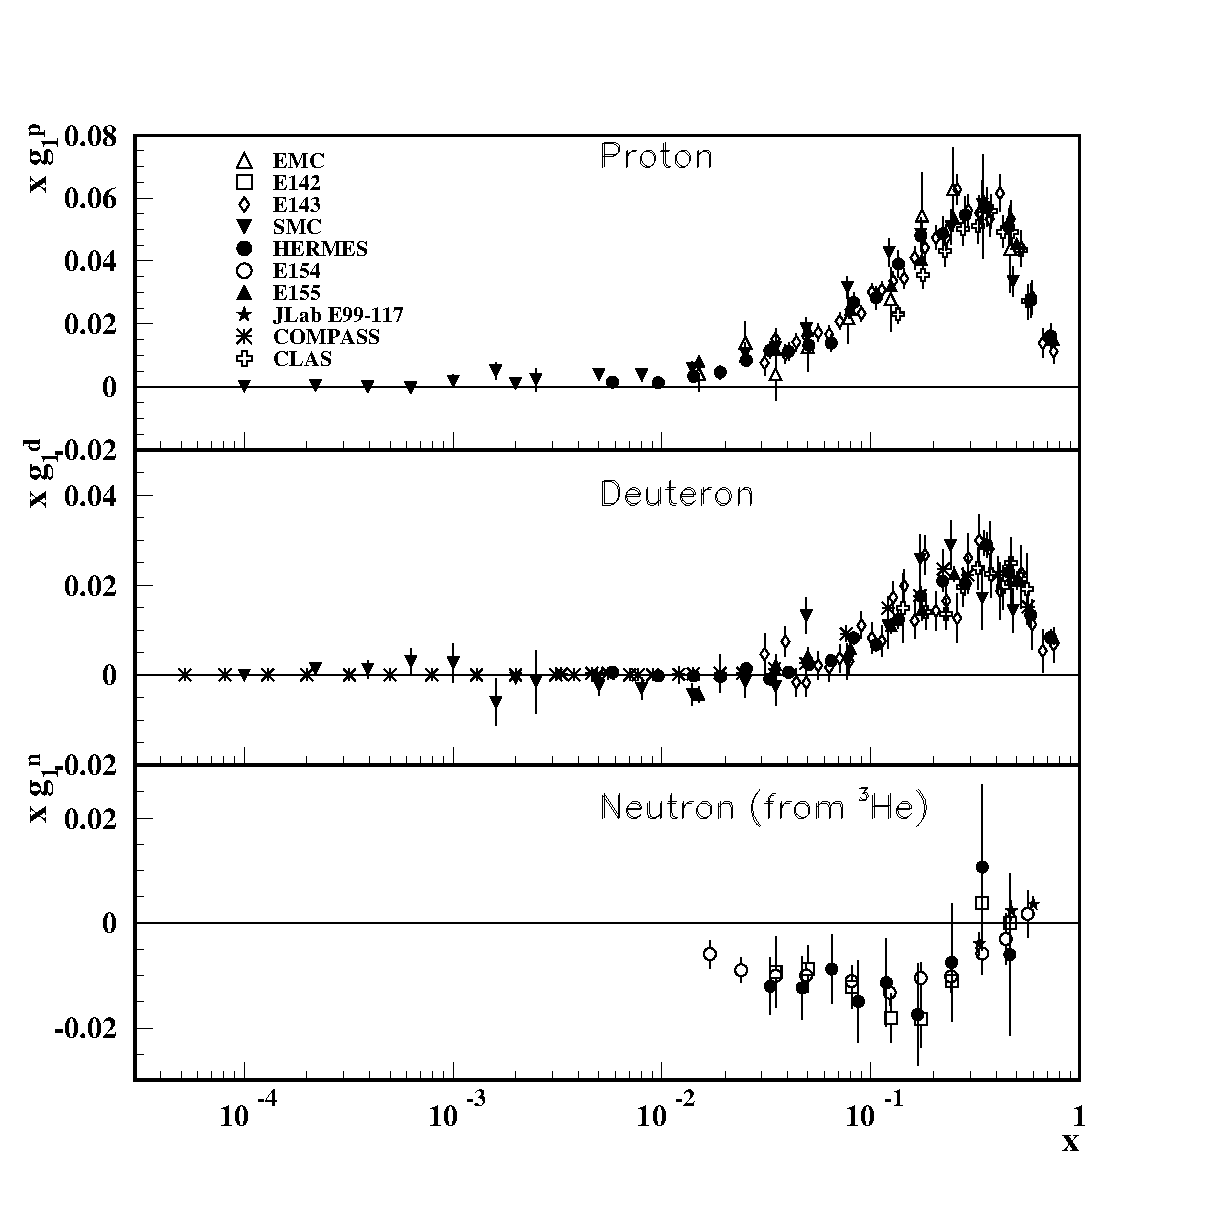
\includegraphics[width=1.0\textwidth]{figures/g1vsx}
%   \caption{World data on the $g_1$ structure functions of the proton, neutron, and deuteron \cite{Amsler:2008zzb}}
%   \label{fig:g1vsx}
% \end{figure}

% \begin{figure}
%   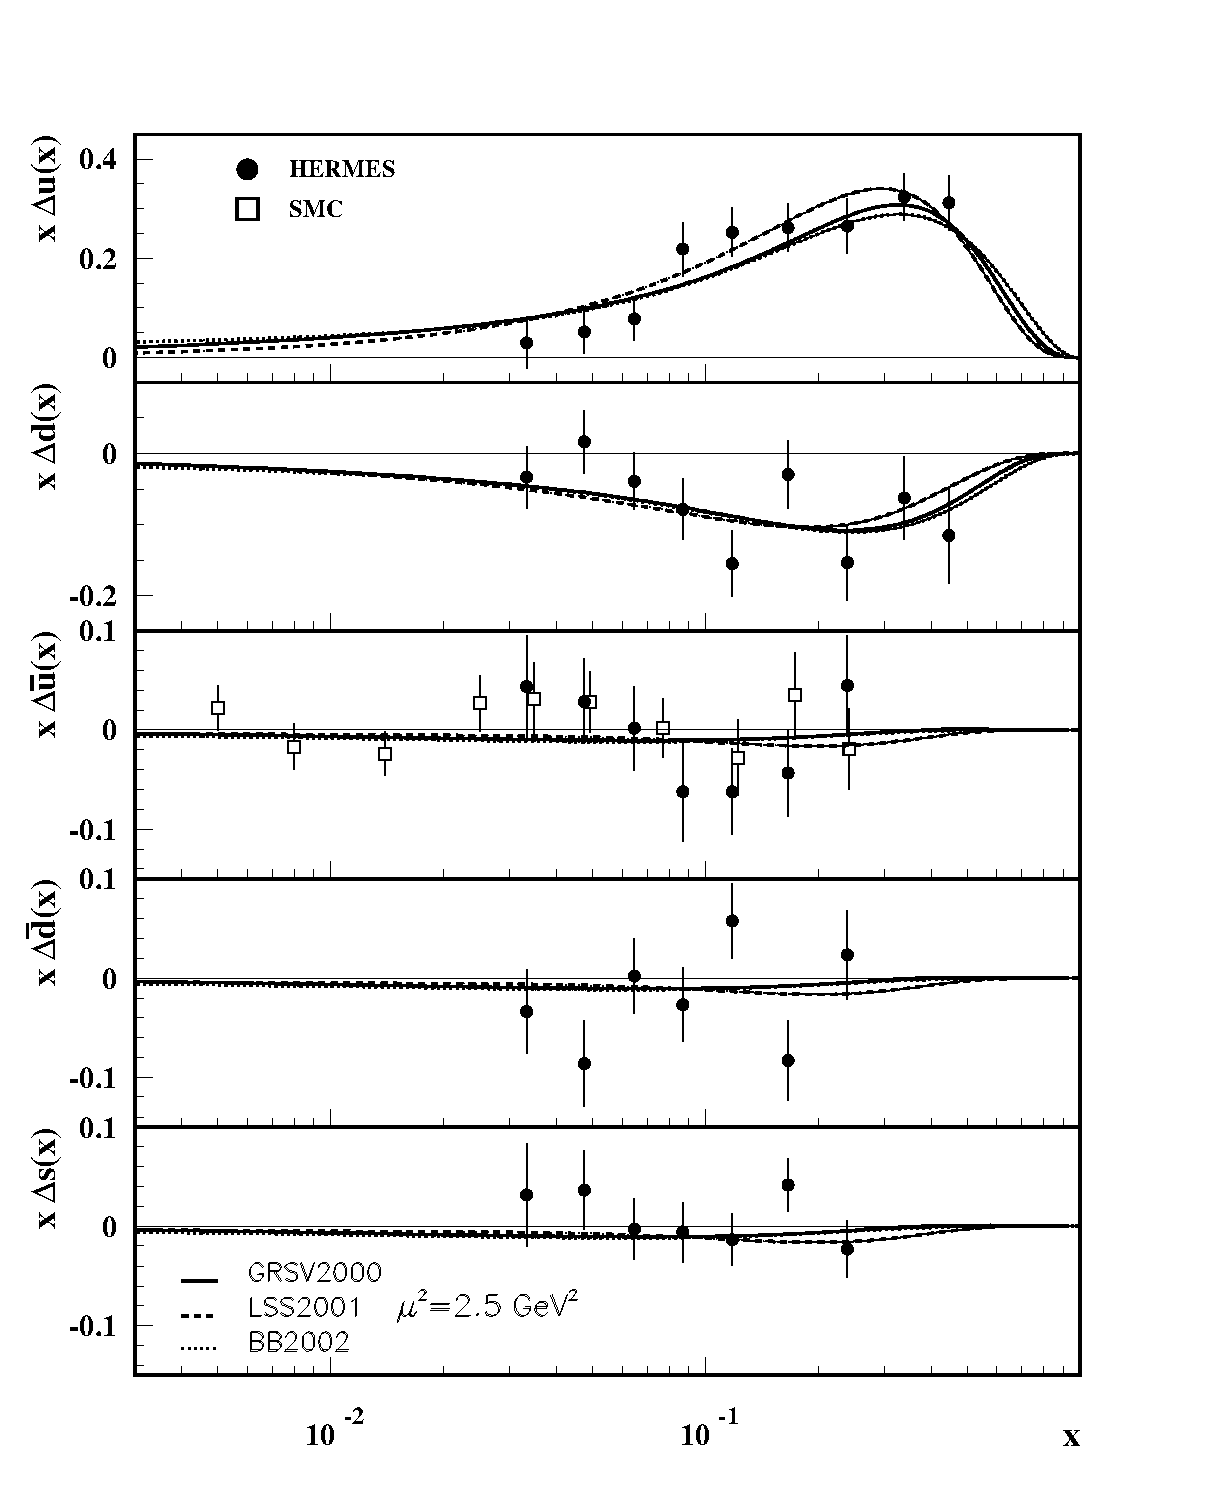
\includegraphics[width=1.0\textwidth]{figures/pol_pdf_5}
%   \caption{from the Particle Data Group \cite{Amsler:2008zzb}.  Data points are SIDIS measurements using positron (HERMES) and muon (SMC).  SMC results extracted assuming $\Delta \bar u(x) = \Delta \bar d(x)$}
%   \label{fig:pol_pdf_5}
% \end{figure}

% \begin{figure}
%   \includegraphics[width=1.0\textwidth]{figures/aac03}
%   \caption{\cite{Hirai:2003pm}  BB \cite{Bluemlein:2002be} uses ISET=3, LSS \cite{Leader:2001kh} uses $\bar{MS}$, GRSV \cite{Gluck:2000dy} uses STD.  But this is of course \textit{not} the most recent polarized PDF analysis using only DIS and SIDIS data.  My best guess at that is \cite{Leader:2006xc}}
% \end{figure}

\begin{figure}
  \centering
  \includegraphics[width=0.6\textwidth]{figures/lss06_deltag}
  \caption{Extraction of the polarized gluon distribution from an analysis of
  scaling violations in DIS and SIDIS. The gray band indicates statistical and
  systematic uncertainties summed in quadrature. Analyses assuming positive,
  negative, and sign-changing gluon polarization all resulted in a comparable
  goodness-of-fit \cite{Leader:2006xc}}
\end{figure}

% Need to understand what constraints go into positive/negative/sign-changing $\Delta g(x)$ parameterizations.
